\documentclass{scrreprt}
\usepackage{enumitem}
\usepackage{listings}
\usepackage{underscore}
\usepackage[ddmmyyyy]{datetime}
\renewcommand{\dateseparator}{--}
\usepackage[bookmarks=true]{hyperref}
\usepackage[utf8]{inputenc}
\usepackage[english]{babel}
\usepackage{url}
\usepackage{graphicx}
\usepackage{tabu}


\newenvironment{enum}
{\begin{enumerate}[label*=\arabic*.][resume]}
{\end{enumerate}}

\hypersetup{
    bookmarks=false,    % show bookmarks bar?
    pdftitle={Test Cases Document},    % title
    pdfauthor={Preet Patel, Matt Horger, John Zlotek},                     % author
    pdfsubject={TeX and LaTeX},                        % subject of the document
    pdfkeywords={TeX, LaTeX, graphics, images}, % list of keywords
    colorlinks=true,       % false: boxed links; true: colored links
    linkcolor=blue,       % color of internal links
    citecolor=black,       % color of links to bibliography
    filecolor=black,        % color of file links
    urlcolor=purple,        % color of external links
    linktoc=page            % only page is linked
}%
\def\myversion{2.0.0 }
\date{}
%\title
\usepackage{hyperref}
\begin{document}

\begin{flushright}
    \rule{16cm}{5pt}\vskip1cm
    \begin{bfseries}
        \Huge{Software Validation \& Test Cases\\Document}\\
        \vspace{1.0cm}
        for\\
        \vspace{1.0cm}
        Checkers\\
        \vspace{1.5cm}
        \LARGE{Version \myversion}\\
        \vspace{1.5cm}
        Prepared by:\\
    John Zlotek\\
    Matt Horger\\
    Jake Carfagno\\
    Preet Patel\\
        \vspace{1.9cm}
        Team: \textbf{Big Chungus}\\
        \vspace{1cm}
        \today\\
    \end{bfseries}
\end{flushright}

\tableofcontents

\chapter*{Revision History}

\begin{center}
    \begin{tabular}{|c|c|c|c|}
        \hline
        Name & Date & Reason For Changes & Version\\
        \hline
        1.0.0 & \formatdate{12}{8}{19} & Initial Draft & pp534\\
       \hline
        2.0.0 & \formatdate{14}{8}{19} & Final Draft and Revisions & mh3294\\
        \hline
    \end{tabular}
\end{center}

\chapter{Introduction}

\section{Purpose of Document}
The purpose of this document to document and demonstrate that our Checkers game design and functionality
aligns with the requirements outlined in the referenced requirement document. This document includes validation and testing
of all possible scenarios by defining accepting states and noting the actual outcome of each respective case.

\section{Scope of Document}
The scope of this document encompasses the three phases that are each unique parts in our overall game procedure. We chose to separate our tests into three phases because they are each independent in that they encapsulate similar tests, yet are dependent on each other via a linking action or procedure.
This document will try to justify that our design has been tested and meets the entire specifications of our requirements, and will report any bug that exists within our testing suite.

\section{References}
All required references can be found in the preceding document at the terminal end. Most of these references will point towards are design and requirements document, which have been previously submitted.

\chapter{Testing Environment}
This section has brief information about the system environment where the test suite was performed and the
information of the tester.

\section{Developer's Environments}

\begin{center}
	\begin{tabular}{|l|l|l|l|l|l|}
	\hline
  	Machine Name & OS & Client/Server & JRE & Person & Date \\
 	\hline
          patel_laptop & MacOS & Client & Java 12 & Patel,P & \formatdate{12}{8}{19}\\
          \hline
          horger_desktop & Windows 10 & Server & Java 12 & Horger,M & \formatdate{14}{8}{19}\\
          \hline
          zlotek_laptop & Ubuntu and Arch Linux & Server & Java 12 & Zlotek,J & \formatdate{19}{8}{19}\\
          \hline
          carfagno_desktop & Windows 10 & Client & Java 12 & Carfagno, J & \formatdate{19}{8}{19}\\
         \hline

	\end{tabular}
\end{center}

\chapter{Testing Environment Setup and Prerequisites}

Prerequisite
\begin{itemize}
  \item This game has implemented a Java Swing GUI for interaction. Java 12.0 is needed on the target system in order for the user to properly see the UI without any issues.
  \item Just for testing purpose, our program can be tested on a single, localhost machine. For multiplayer games with other devices, a stable Internet connection is needed.
  \item A Drexel Account is required to interact with the lobby structure to satisfy the tests conditions.
\end{itemize}

\chapter{Test Cases}

This chapter is divided into four sections, each respective to each phase of the game. The first phase includes the launching portion of the game, as well as interacting with the key menus to launch lobbies. The second phase tests the validation and logic of gameplay. The Third phase, while small, tests the functionality of multiple sessions running concurrently in conjuncture with the server. Finally, the fourth phase tests win conditions and outlying cases. If a test is Work-In-Progress, this means we are crafting the test suite or finalizing the components used in the testing mechanism.

\section{Test Phase 1: Starting Game}

\subsection{Description}
This section covers the testing of the initial phase of launching the program, creating a lobby, joining a lobby and starting a new game. This section relies heavily on UI interaction with our Swing menus.
\subsection{Prerequisites for this test case} An internet connection with a firewall rule allowing traffic on all ports, to be certain, is required to this phase. Localhost also works just fine, as long as two sessions are able to run on the target machine with no drawbacks.
\subsection{Scenario}

\begin{tabu} to \textwidth {| c | X | X | X | X | X |}
\hline
\textbf{Item No.} & \textbf{Case} & \textbf{Expectation} & \textbf{Actual Outcome} & \textbf{Requirement Reference}\\ \hline
1 & Launch the game with active internet connection & GUI of Lobby menu should be launched & Passed & R1.1 \\ \hline
2 & Launch the game with server down & GUI Warning should be present & Passed & R1.2 \\ \hline
3 & Launch the game with no active internet connection & GUI Warning should be present & Failed, GUI not developed & N1.1 \\ \hline
4 & Launch the game outside of Drexel's internet connection & GUI Warning should be present & Work-In-Progress & N1.2 \\ \hline
5 & Create a lobby button clicked & Create a lobby ID & Passed  &L1.1 \\ \hline
6 & Join a lobby button clicked & Once lobby selected from lobby menu, player should be able to join that session & Passed &L1.1 \\ \hline
7 & Create multiple sessions & No more then 10 lobbies should be allowed & Work-In-Progress &L2.2\\ \hline
8 & Start 5 lobbies concurrently with 10 clients & There should be no warning present &  Passed &L2.3\\ \hline
9 & Start 10 lobbies with 11 clients & 11th player should not able to create a lobby & Work-In-Progress &L2.3\\ \hline
10 & Initialize Lobby with 2 clients & GUI should have 8X8 board with randomly assigned color for clients  & Passed &G1 \\ \hline
11 & Client tries to connect to lobby with an invalid ID  & GUI Warning should be present & Failed, GUI not developed & L2.6\\ \hline
\end{tabu}
\newpage


\section{Test Phase 2: Gameplay Validation}

\subsection{Description}
This section covers the testing of the gameplay validation system. This includes the testing of game moves, moves that are valid and invalid, jumps, and the process of king generation. These requirements to which they match up are mostly in the 6.2 Gameplay section of our requirements documentation. Finally, we want to make the distinction that we want to test the end-facing client, because that is the product we are sending as our deliverable. 

\subsection{Prerequisites for this test case}
A valid lobby that has been initialized for an in-progress game. Note, we will be talking about the server validation of clients disconnecting and other similar processes in the next phase. For reference, we will be posting a picture of the board below, so you, the reader, can have a graphical representation to what we are talking about.

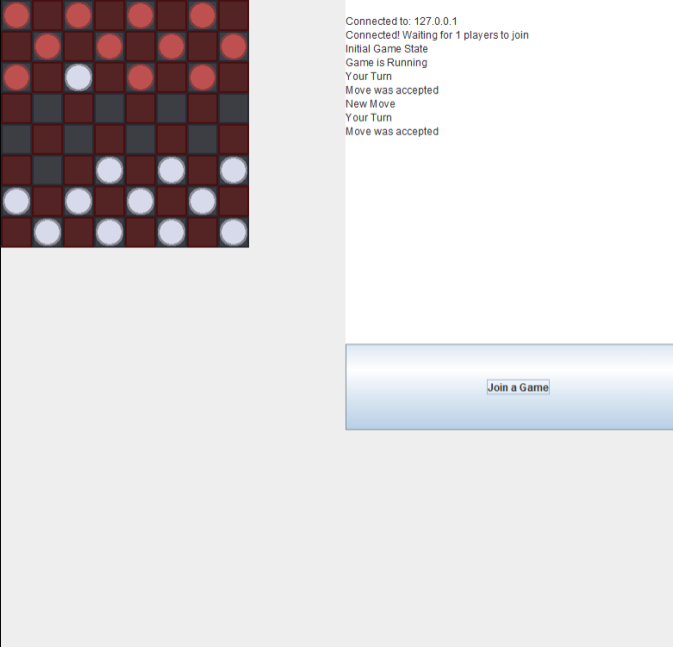
\includegraphics[scale=0.7]{board.png}

\subsection{Scenario}
\begin{tabu} to \textwidth {| c | X | X | X | X | X |}
\hline
\textbf{Item No.} & \textbf{Case} & \textbf{Expectation} & \textbf{Actual Outcome}  & \textbf{Requirement Reference}\\ \hline
1 & Black piece first move & Only player with black piece should make move &  Passed  &G4\\ \hline
2 & White piece makes the first move & If Player with white piece makes the move, then it should be discarded and the piece should come back to the original position &  Passed  &G2\\ \hline
3 & Piece makes a move & Can move diagonally in either direction and piece stays in new square &  Passed  &G5\\ \hline
4 & Non-crowned piece tries to jump & Only jump and capture the opponent piece if there is an empty square above that targeted piece. &  Passed  & G5 \\ \hline
\end{tabu}
\newpage
\begin{tabu} to \textwidth {| c | X | X | X | X | X |}
\hline
\textbf{Item No.} & \textbf{Case} & \textbf{Expectation} & \textbf{Actual Outcome} & \textbf{Requirement Reference}\\ \hline
5 & Non-crowned piece tries to jump multiple & If a jump is made over multiple piece against opponent with respect to 4, move is valid. &  Passed  &G5 \\ \hline
6 & Non-crowned piece tries to not move diagonally & If a piece move in horizontal or vertical direction then it should come back to original position & Passed  &G5 \\ \hline
7 & Non-crowned piece moves backwards & If a piece tries to move backward diagonally, then it should be discarded and it should come back to original position &  Passed  &G5 \\ \hline
8 & Non-crowned piece has no space for jump & if there is not space to place the piece after the jump to capture, then it should come back to original position &  Passed  &G5 \\ \hline
9 & Non-crowned piece has no space for multiple jump & If jump made over player's own piece is valid, and next jump is not, only prompt the first jump  &  Passed  &G5 \\ \hline
\end{tabu}
\newpage
\begin{tabu} to \textwidth {| c | X | X | X | X | X |}
\hline
\textbf{Item No.} & \textbf{Case} & \textbf{Expectation} & \textbf{Actual Outcome} & \textbf{Requirement Reference}\\ \hline

10 & Non-crowned piece turns into king & If either player piece reaches to the 10th row from player direction then, piece should turn into a crowned piece &  Passed  &G6 \\ \hline
11 & Crowned piece makes a move & A crown can move in any four diagonal direction & Passed  &G6 \\ \hline
12 & Crowned piece makes a jump & A crown can jump in any direction as long as test case 4 is valid  & Passed  &G6 \\ \hline
13 & Crowned piece makes multiple jumps & A crown can jump in any direction as long as test case 12 is true & Passed &G6 \\ \hline
14 & Crowned piece tries to not move diagonally & A crown cannot move  horizontal or vertical; piece should return in original direction & Passed  &G6 \\ \hline
15 & Crowned piece makes an invalid jump & If a jump is made over a player's own piece, the piece should return in original direction &  Passed  &G6 \\ \hline
16 & Crowned piece placed in the 10th row again & The crown piece state should not be affected in any way &  Work-In-Progress  & G6\\ \hline
\end{tabu}


\section{Test Phase 3: Multiple}

\subsection{Description}
This section covers the testing of the proper game performance of multiple sessions running at the same time. Most of our server tests are in this phase below, as they are independent of the client tests. The cases where they match are detailed in the final phase, along with the win conditions.

\subsection{Prerequisites for this test case}
More than one game lobby running for these tests to work. An active server must also be running on Drexel's network in order to properly achieve network results.

\subsection{Scenario}
\begin{tabu} to \textwidth {| c | X | X | X | X | X |}
\hline
\textbf{Item No.} & \textbf{Case} & \textbf{Expectation} & \textbf{Actual Outcome} & \textbf{Requirement Reference}\\ \hline
1 & Lobby only sends activity between two fixed clients & Only changes in the game state should be seen between two clients and should not interfere other session game play &  Work-In-Progress  & L2.3 \\ \hline
2 & Client has poor network connection & Server should automatically alert the client connection &  Work-In-Progress  & N1.4\\ \hline
3 & Client can't connect to the server within a reasonable time & Server should automatically close the requested connection & Passed & N2.4 \\ \hline
4 & Server shuts down unexpectedly & All lobbies are warned gracefully of the shutdown & Failure - need error handling & L2.4 \\ \hline
5 & Lobby concludes the game & No other lobbies should be opened or closed in any way & Passed & L2.5 \\ \hline
6 & Server starts back up after it terminated with lobbies active & No lobbies will be re-created as clients have disconnected & Work-In-Progress & N2.3 \\ \hline
\end{tabu}

\section{Test Phase 4: Ending the game}

\subsection{Description}
This section covers the testing of the scenario when the game ends and all possibilities of further action that can be taken from the clients.

\subsection{Prerequisites for this test case}
At least one lobby in the active state, with the game in progress. Two clients are required for each of these test cases.

\subsection{Scenario}
\begin{tabu} to \textwidth {| c | X | X | X | X | X |}
\textbf{Item No.} & \textbf{Case} & \textbf{Expectation} & \textbf{Actual Outcome} & \textbf{Requirement Reference}\\ \hline
1 & Piece makes a winning jump & If a piece makes a valid jump over the last piece, then that player should be declared the winner &  Passed  &6.2.1 \\ \hline
2 & Game Concludes & Player who won should receive the winner message, loser should receive the opposite message & Work-In-Progress  &6.2.1 \\ \hline
3 & Client want to leave the lobby & Once a client quits the lobby, they should be returned to the lobby screen&  Passed  &6.2.2 \\ \hline
4 & Client leaves the lobby & The other connected client to the lobby is declared the winner  & Work-In-Progress  &6.2.2 \\ \hline
5 & After game is finished, both players want a rematch & A new lobby will be created with the same two clients & Failed - throwing errors  &6.2.2 \\ \hline
6 & After game is finished, if one player doesn't want a rematch & Both players will return to the lobby screen & Work-In-Progress & 6.2.2\\ \hline
\end{tabu}

\begin{thebibliography}{9}

\bibitem{referenceDocument}
  Team Big Chungus,
  \textit{Software Requirements Specification},
 CS 451-002, Drexel University,
  Summer 2019.

\bibitem{designDocument}
Team Big Chungus,
\textit{Software Design Document},
 CS 451-002, Drexel University,
  Summer 2019.


\end{thebibliography}


\end{document}
